\chapter{Anwendungen}
\label{Anwendungen}

In diesem Kapitel wird beschrieben, wie Pfadplanung Algorithmen in realen Anwendungen eingesetzt werden können.
\section{GIS(Geoinformationssystem)}
\label{GIS(Geoinformationssystem)}
% \subsection{Definition}

Ein geografisches Informationssystem (GIS) ist ein System zum Erstellen, Verwalten, Analysieren und Kartieren verschiedener Arten von Daten. GIS verknüpft Daten mit einer Karte und integriert Standortdaten mit verschiedenen Arten von beschreibenden Daten. Dies ist die Grundlage für die Kartierung und Analyse in der Wissenschaft und in fast allen Branchen.
Bei diesen Daten handelt es sich um Informationen über Objekte auf der Erde wie Städte, Eisenbahnstrecken, Flüsse usw \cite{Vaibhavi2014}. 

% \subsection{Geoinformationssystem mit Dijkstra-Algorithmus}
Algorithmen für den kürzesten Weg werden in Kartenplattformen wie Google Maps verwendet, um den kürzesten Weg zwischen zwei Punkten zu ermitteln.
Obwohl der Dijkstra-Standardalgorithmus in diesem Fall anwendbar zu sein scheint, dauert das Routing des Pfades vom Startpunkt zum Endpunkt in einer großen Datenmenge sehr lange \cite{HamidAli2020}.

 Um bei der Berechnung des kürzesten Weges Zeit zu sparen und eine bessere Lösung zu erhalten. Beeinflusst von \cite{HamidAli2020}, der bessere Ansatz besteht darin, vor dem Start des Dijkstra-Algorithmus einen temporären Datensatz zu erstellen und ihn so zu behandeln, als wäre er der Graph, mit dem der Algorithmus arbeiten muss. 
 Nachdem die Start- und Endknoten ermittelt wurden, wird dieser Datensatz erstellt. Der Datensatz kann anhand der Koordinaten des Start- und des Zielknotens aus den Hauptdaten ausgeschlossen werden, indem nur die Knoten ausgewählt werden, die sich innerhalb des von den beiden Knoten gebildeten Quadrats befinden.
 Es gibt andere Algorithmen, die in GIS verwendet werden können, um bessere Ergebnisse zu erzielen, wie z. B. A*.


\newpage
\section{Mobile Roboter}
\label{Mobile Roboter}
Mit der Weiterentwicklung der Internet-of-Things-Technologien in den letzten Jahren hat die Entwicklung intelligenter Städte in der Industrie große Aufmerksamkeit erlangt.
Die Steuerung mobiler Roboter ist ein wichtiges Thema in intelligenten Städten und die Pfadplanung ist eine wichtige Komponente unter den mobilen Roboter-Technologien, die dem Roboter hilft, den Weg von einem Startpunkt zu einem Zielpunkt zu finden und dabei sicher und zuverlässig alle Hindernisse in einer statischen und dynamischen Umgebung während der Reise zu vermeiden \cite{Myung21,Hong-mei17}.

\subsection{Umgebungsmodell}
Das Rolling-Window-Prinzip wird zur Hindernisvermeidung in einer unbekannten Umgebung verwendet, während die Algorithmen Dijkstra und A* in erster Linie für die Pfadplanung in einer bekannten Umgebung eingesetzt werden.
\newline
Da sowohl der Dijkstra- als auch der A*-Algorithmus Gitter-basierte Suchmethoden sind, sollte zunächst das Gittermodell der umgebenden Karte erstellt werden. Bei der Gittermethode wird die Karte in benachbarte Gitter gleicher Größe unterteilt. 
Die Größe des mobilen Roboters bestimmt die Größe des Gitters und beeinflusst die Suchgenauigkeit und Effizienz des Algorithmus \cite{Hong-mei17}.
\newline
Das Gittermodell einer Umgebungskarte ist in der Abbildung \ref{fig:Umgebungsmodell-Grid} unten dargestellt.

\begin{figure}[H]
	\centering
	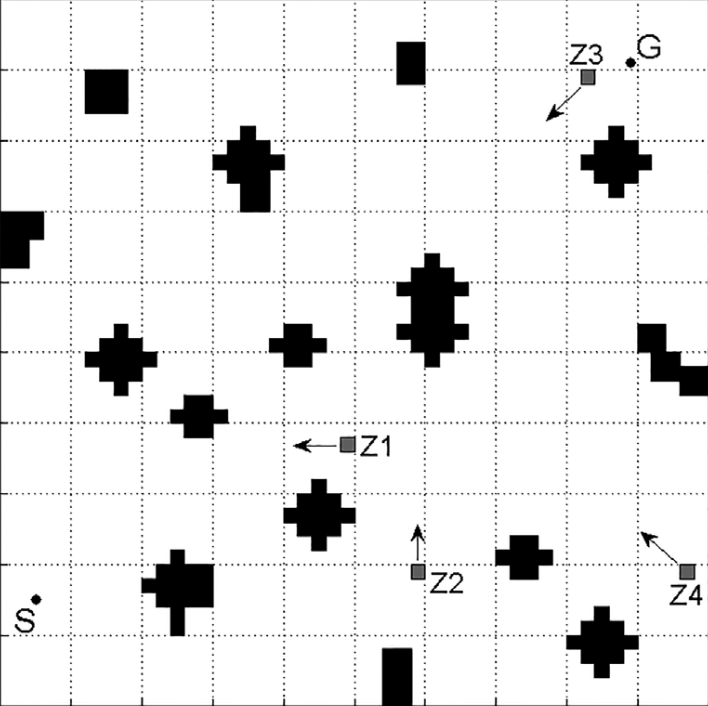
\includegraphics[width=0.5\textwidth]{images/Grid_Modell.PNG}
	\caption{Umgebungsmodell angelehnt an \cite{Hong-mei17}.}
	\label{fig:Umgebungsmodell-Grid}
\end{figure}

\subsection{Dijkstras Algorithmus und A*-Algorithmus}

Die Idee ist, A*- und Dijkstra-Algorithmen miteinander zu kombinieren, um die Effizienz der Planung einer idealen kollisionsfreien Route für einen mobilen Roboter zu erhöhen. Bei der Neuplanung wird die Dijkstra-Methode zur Vorverarbeitung der statischen Umgebungskartendaten angewendet, die optimale Routen vom Ziel G zu allen freien Zuständen plant und speichert. Wenn der Roboter auf seinem Weg zum Ziel auf ein bewegliches Hindernis trifft, wählt das Rolling-Window-Prinzip einen lokal optimalen Zustand als nächsten Zielzustand. Dann wird mit dem A*-Algorithmus eine lokal optimale Route von der Roboterposition zum lokalen Ziel neu geplant.
Die neue Route kann den Roboter um Hindernisse herumführen \cite{Hong-mei17}.



\section{Autonome Navigation}
\label{Autonome Navigation}

Pfadsuchalgorithmen werden ebenfalls im Bereich des Autonomen Fahrens, oder auch bei unbemannten Flugfahrzeugen verwendet
um sichere, effiziente, kollisionsfreie und kostengünstige Wege von Start zum Ziel zu führen, was die Wahl des richtigen Pfadsuchalgorithmen
zu einer wichtigen Aufgabe macht. Es hängt unter anderen Faktoren die Geometrie des Fahrzeugs von dieser Wahl ab \cite{Karur:21}.
Mit der zunehmenden Verbreitung von autonomen Fahrzeugen, die immer mehr Wegfindung und -planung erfordert, sind Pfadsuchalgorithmen
zu einem neuen Schwerpunkt der autonomen Steuerung geworden \cite{Karur:21}.
Da mobile Roboter in vielen Anwendungen eingesetzt werden, haben Forscher Methoden entwickelt, um die 
Anforderungen an mobile Roboter effektiv erfüllen zu können und einige Herausforderungen für die Umsetzung einer vollständig oder
teilweise autonomen Navigation in unübersichtlichen Umgebungen zu bewältigen \cite{Karur:21}.
So wird die Wahl des richtigen Pfadplanungsalgorithmus von der kinematischen Bewegungsgestaltung des Roboters/Fahrzeugs,
den zur Verfügung stehenden Rechenressourcen, sowie der sensorischen Ausstattung des Fahrzeugs bestimmt \cite{Karur:21}.

Die Leistung und Komplexität des verwendeten Algorithmus hängt auch vom Anwendungsfall ab \cite{Karur:21}.

Somit gibt es nicht \emph{den perfekten Pfadsuchalgorithmus für Autonomes Fahren}, aber es finden viele verschiedene Algorithmen eine 
Anwendung in der autonomen Navigation.